\documentclass[11pt, oneside]{article} 
\usepackage{geometry}
\geometry{letterpaper} 
\usepackage{graphicx}
	
\usepackage{amssymb}
\usepackage{amsmath}
\usepackage{parskip}
\usepackage{color}
\usepackage{hyperref}

\graphicspath{{/Users/telliott_admin/Tex/png/}}
% \begin{center} 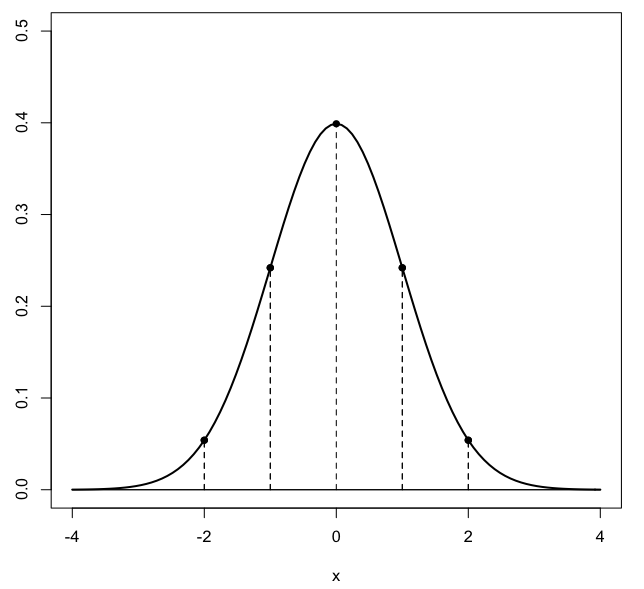
\includegraphics [scale=0.4] {gauss3.png} \end{center}

\title{Value of pi and Gregory}
\date{}

\begin{document}
\maketitle
\Large
\label{sec:Gregory}

As discussed in a previous \hyperref[sec:Archimedes_and_pi]{\textbf{chapter}}, Archimedes used paired inscribed and circumscribed polygons to come up with an iterative procedure that one can use to calculate the value of $\pi$ \emph{to any desired accuracy}.  

As an engineer, Archimedes knew when to stop, at about $3.1416$.

In our analysis, simple geometry was used to show that for a circle of unit diameter and a polygon of $n$ sides, the inside perimeter is $n \sin \theta$ and the outside perimeter is $n \tan \theta$, where $\theta$ is $2 \pi$ divided by $n$.  

Progression from $n$ sides to $2n$ sides requires the sum of angles theorem to generate new values for the sine and tangent, as well as multiplication by $2$ to account for doubling the number of sides.

The sum of angles gives the following relationships (where the prime designates $2n$ sides and a central angle of $\theta/2$):

\[ C' = \sqrt{\frac{1}{2}(1 + C)} \]
\[ S' = \frac{S}{2C'} \] 
\[ T' = \frac{S}{1 + C} \]
From the last it follows easily that
\[ T' = \frac{ST}{S + T} \]

We can recast these results in terms of the two perimeters $p$ and $P$:
\[ P = nT  \]
\[ P' = 2nT' \]

Substituting for $T'$ in the latter
\[ P' = 2nT' = 2n \ [ \  \frac{ST}{S + T} \ ] \]
\[ = 2 \ [ \frac{nS \cdot nT}{nS + nT} \ ] \]
\[ = 2 \frac{pP}{p + P} \]
The new outside perimeter $P'$ is the harmonic mean of the two perimeters for $n$ sides.

For the second one, $p'$:
\[ S' = \frac{S}{2C'} = \frac{S}{2} \ \frac{T'}{S'} \]
Hence
\[ [2S']^2 = S \cdot 2T' \]
\[ [2nS']^2 = nS \cdot 2nT' \]
so
\[ p'^2 = pP' \]
\[ p' = \sqrt{pP'} \]

$p'$ is the geometric mean of $p$ and $P'$.

That's a summary of what we found before.

On the very same day that I was revising the previous chapter to better integrate these two approaches, I came across another page which gives a "proof without words" of Gregory's Theorem.

\url{https://divisbyzero.com/2018/09/28/proof-without-word-gregorys-theorem/}

It contains the following two formulas:
\[ I_{2n} = \sqrt{I_n C_n} \]
\[ C_{2n} = \frac{2}{1/I_{2n} + 1/C_n} \]

These look very familiar, yet careful comparison shows they are not the same as what we just had above:
\[ p' = \sqrt{pP'} \]
\[ P' = 2 \frac{pP}{p + P} \]

If we were to try to equate $p$ and $I$, as well as $P$ and $C$, we would find two additional primes in the wrong places.  What's going on?

The resolution is that the new formulas relate to the enclosed \emph{areas}, and somehow, the formulas work out almost but not quite the same as those for the corresponding perimeters.

\subsection*{Lemmas}
Given my history with this problem, and the allure of a "proof without words", I was motivated to understand the approach based on areas, so that's what the rest of this chapter is about.

To begin with, the original statements are massaged to form two Lemmas.  These Lemmas are what we will prove by our geometric analysis, below.

The first Lemma is
\[ \frac{I_{2n}}{I_n} = \frac{C_n} {I_{2n}} \]
Our first equation is
\[ I_{2n} = \sqrt{I_n C_n} \]
\[  I_{2n} \cdot I_{2n} = I_n C_n \]
The result follows easily.

The second one is
\[ \frac{C_n - C_{2n}} {C_{2n} - I_{2n}} = \frac{C_n}{I_{2n}} \]

This was quite a bit more challenging, so much so that I substituted symbols and then pushed those symbols around for some time before seeing the answer.  We were given
\[ C_{2n} = \frac{2}{1/I_{2n} + 1/C_n} \]
This can also be written as
\[ \frac{2}{C_{2n}} = \frac{1}{I_{2n}} + \frac{1}{C_n} \]

Four steps for the hard part.  First, clear all three denominators
\[ 2 C_n I_{2n} = C_n C_{2n} + C_{2n} I_{2n} \]
Split up the two copies of $C_n I_{2n}$:
\[  C_n I_{2n} - C_{2n} I_{2n} = C_n C_{2n} - C_n I_{2n} \]
Factor
\[  I_{2n}(C_n - C_{2n}) = C_n (C_{2n} - I_{2n}) \]

Lastly, form the ratios:
\[ \frac{C_n}{I_{2n}} = \frac{C_n - C_{2n}}{C_{2n} - I_{2n}} \]
which is what was to be proved.

$\square$

\subsection*{proof without words}
We start the geometry by drawing the arc of one-sixth of a circle, together with the inscribed and circumscribed perimeters.  (This is just a convenient size, the argument does not depend on the size of the arc.)

\begin{center} 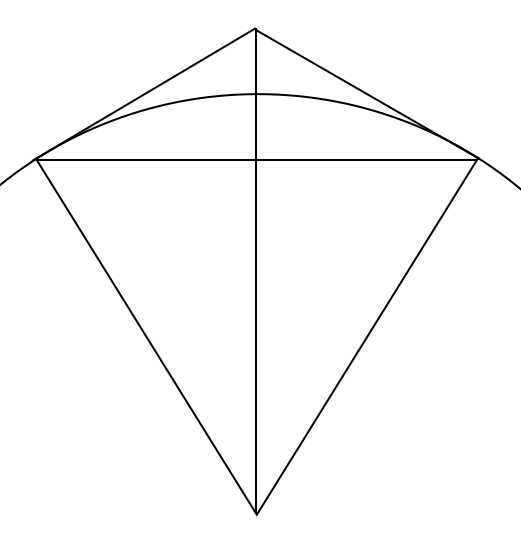
\includegraphics [scale=0.3] {Gregory0.png} \end{center}

We proceed to find expressions for the areas corresponding to $I_n, I_{2n}, C_n, C_{2n}$.  Three of these are easy, but the last is more difficult.  It is really the heart of the proof.

The first is $I_n = nca$:
\begin{center} 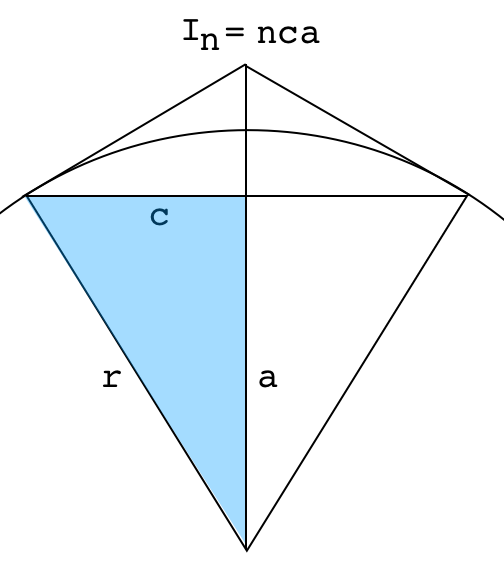
\includegraphics [scale=0.3] {Gregory1.png} \end{center}
Two copies of a triangle of base $a$ and height $c$, times the number of sectors.

The second is $I_{2n} = ncr$:
\begin{center} 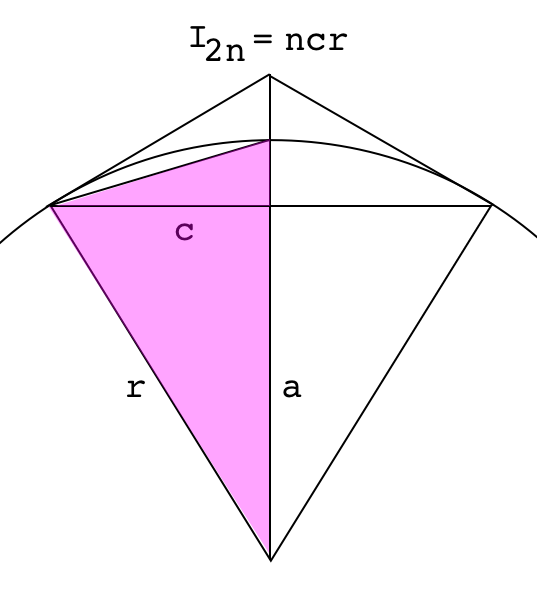
\includegraphics [scale=0.3] {Gregory2.png} \end{center}
If you focus on the left-hand side, this one looks wrong at first.  $c$ does not seem to be an altitude of the triangle for which $r$ is the base.  

Two means of resolution:  recognize that the pink triangle is isosceles.  Therefore $c$ is equal to that altitude. Alternatively, see that the base along the central axis is also equal to $r$.
\begin{center} 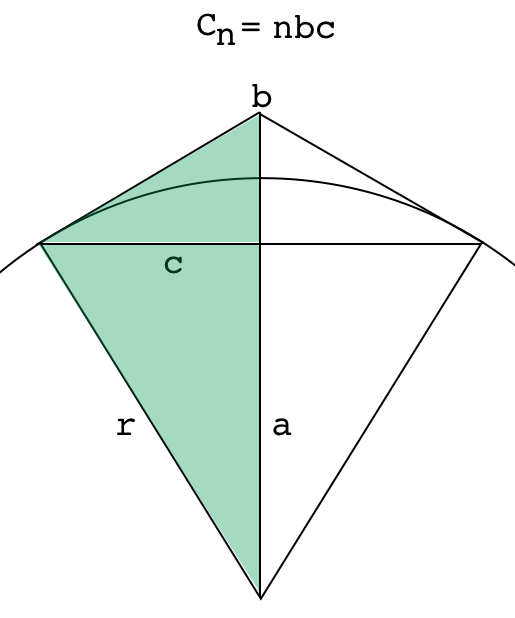
\includegraphics [scale=0.3] {Gregory3.png} \end{center}
Above is $C_n = ncb$:

Recall that the side of the external polygon is tangent to the circle.  

The last one is more complicated:
\begin{center} 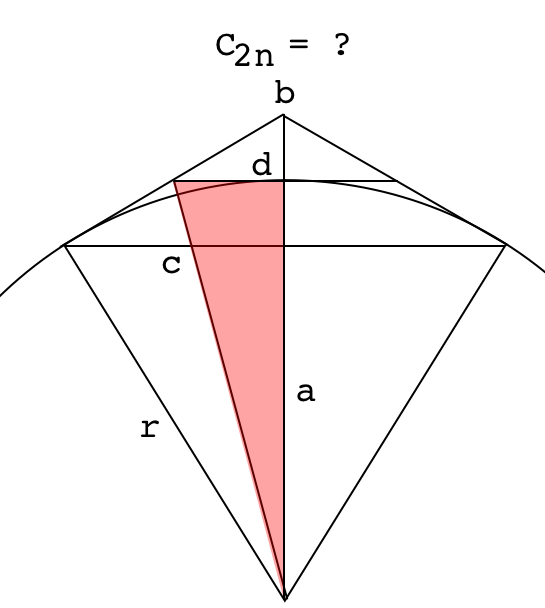
\includegraphics [scale=0.3] {Gregory4.png} \end{center}
We obtain this area as two different differences.

We have this:
\begin{center} 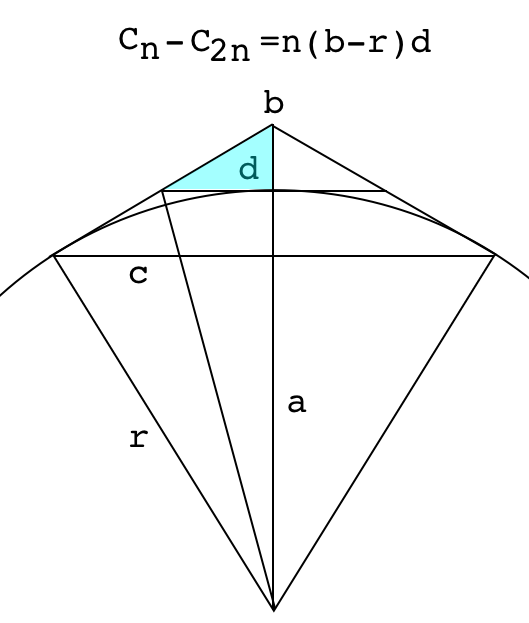
\includegraphics [scale=0.3] {Gregory5.png} \end{center}
and this
\begin{center} 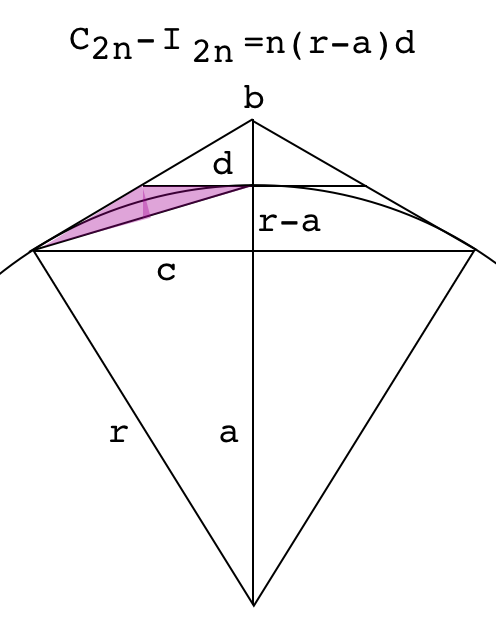
\includegraphics [scale=0.3] {Gregory6.png} \end{center}

\subsection*{resolution}
Recall our Lemmas:
\[ \frac{I_{2n}}{I_n} = \frac{C_n}{I_{2n}} = \frac{C_n - C_{2n}}{C_{2n} - I_{2n}} \]
We can rewrite these in terms of the segments from the circle:

\[ \frac{I_{2n}}{I_n} = \frac{ncr}{nca} = \frac{r}{a} \]
\[ \frac{C_n}{I_{2n}} = \frac{ncb}{ncr} = \frac{b}{r}  \]
\[ \frac{C_n - C_{2n}}{C_{2n} - I_{2n}} = \frac{n(b-r)d}{n(r-a)d} = \frac{b-r}{r-a} \]

If we can prove that these three ratios are all equal to each other, then we're done.  We will have used the geometry to prove the Lemmas, and those can be used in turn to prove the original Gregory formulas.

But this is easy:
\begin{center} 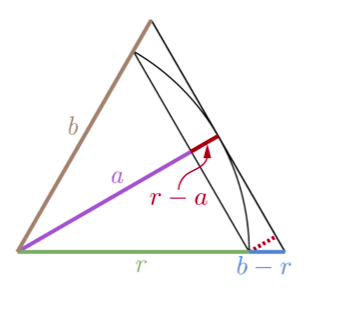
\includegraphics [scale=0.6] {Gregory7.png} \end{center}

It's just a matter of similar triangles:
\[ \frac{r}{a} = \frac{b}{r} = \frac{b-r}{r-a} \]

That's the "without words" part.

$\square$

\subsection*{historical notes}

The area-based formulas given above are due to James Gregory.

\url{https://divisbyzero.com/2018/09/28/proof-without-word-gregorys-theorem/}

As an aside, the Fundamental Theorem of Calculus (FTC) is usually thought about (taught and learned) using the language of functions, and ascribed mainly to Leibnitz, with some credit the two Isaacs, Newton and his teacher, Barrow.

\url{https://arxiv.org/abs/1111.6145}

Amazingly enough, Gregory published a geometric (Euclidean) proof of the FTC in 1668!  That predates Liebnitz (1693) by more than 25 years.  This is another reason why one should attempt to give considerable credit to individuals other than Newton and Liebnitz (Fermat, Pascal, Wallis, Gregory, etc.) in the invention of the calculus.

\subsection*{connection to the perimeters}
It is worth taking another look at our formulas for the perimeters in terms of the geometry we've laid out in this chapter.  We have:
\begin{center} 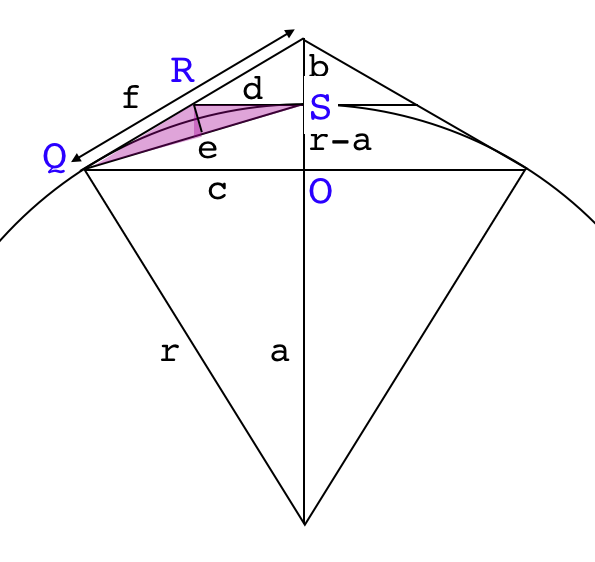
\includegraphics [scale=0.4] {Gregory8.png} \end{center}
where $c$ and $d$ go only across the half-sector (refer back to the area calculation above).

It looks as if the segment of the vertical that extends beyond the radius might be equal to that part below, and above what looks like the "strut" of a kite.  This is not true.  In the notation from the figure
\[ \frac{b-r}{r-a} \ne 1 \]
Instead, it is equal to $r/a$.

Another way to say this is that $QS$ is the angle bisector of the original $\angle RQO$, and in general 
\[ \tan 2 \theta \ne 2 \tan \theta \]
rather
\[ \tan 2 \theta = \frac{2 \tan \theta}{1 - \tan^2 \theta} \]
(although having said that, for small $\theta$, $\tan \theta \approx \theta$ and this is almost correct).

However, the key observation is that the purple triangle is isosceles.  A simple proof is to appeal to the symmetry of the circumscribed polygon.
\begin{center} 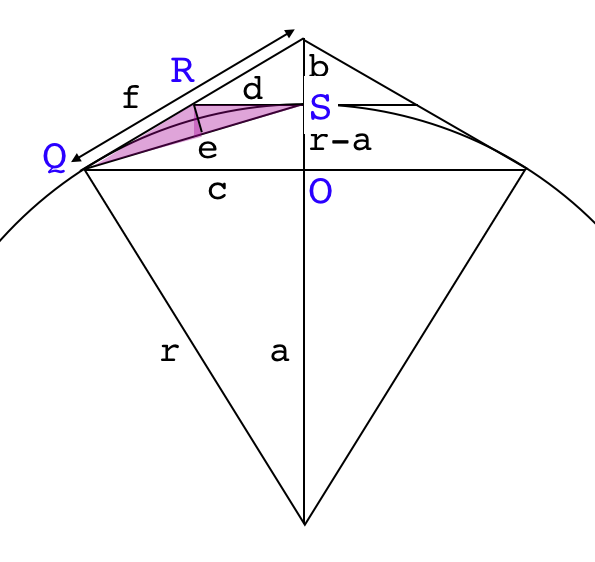
\includegraphics [scale=0.4] {Gregory8.png} \end{center}
Also observe that $\angle SQO = \angle QSR$ by the alternate interior angles theorem.  Therefore the cosines are also equal, namely:
\[ \frac{c}{e} = \frac{e/2}{d} \]
\[ 2dc = e^2 \]

Now, $c$ is the entirety of $p$ in this half-sector.  But $d$ is only one-half of $P'$.  

Hence $2d \cdot c$ is equal to $pP'$, and since $e = p'$, we have that 
\[ pP' = p'^2 \]
which was our first rule for the perimeters.

The second rule was
\[ P' = 2 \frac{pP}{p + P} \]

In geometric terms, we must show that
\[ 2d = 2 \frac{cf}{c + f} \]
\[ cd + df = cf \]

Taking another look at the diagram:
\begin{center} 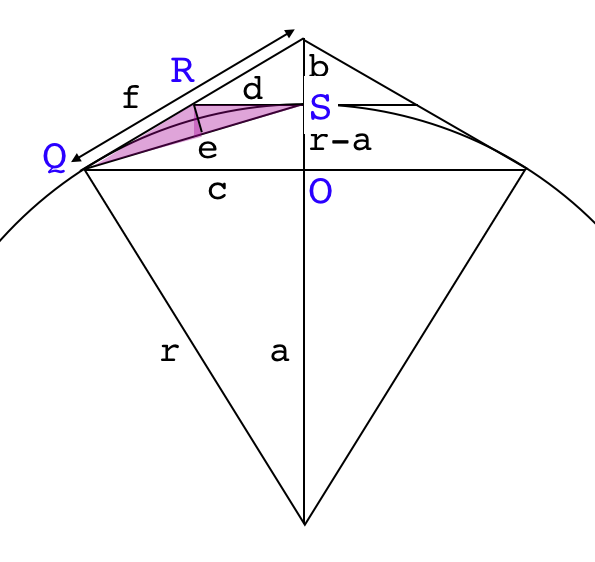
\includegraphics [scale=0.4] {Gregory8.png} \end{center}

The small triangle with base $d$ has slanted side $f - d$ (subtracting $d$ because $\triangle QRS$ is isosceles).  By similar triangles, then, we have
\[ \frac{d}{f-d} = \frac{c}{f} \]
\[ df = cf - cd \]
\[ cd + df = cf \]
But this is what we needed to prove.

$\square$

It's worth noting that the derivation does not depend on the angle chosen for the sector.  

What is important is that the purple triangle is isosceles.  This is guaranteed by the process of drawing two inscribed triangles, one of half the angle than the other, due in turn to the fact that $QS$ is a bisector of $\angle RQO$.

\begin{center} 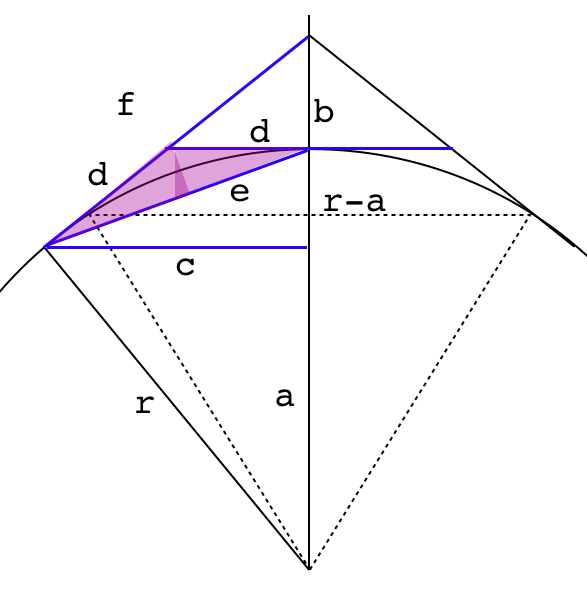
\includegraphics [scale=0.3] {Gregory9.png} \end{center}

We can see this by redrawing the figure with a slightly larger sector.  The original sector is indicated by the equilateral triangle with the dotted line.  The purple triangle is still isosceles.  All the rest follows.

\end{document}